\documentclass[a4paper]{article}
\usepackage[margin=25mm]{geometry}
\usepackage{amsmath}
\usepackage{amsfonts}
\usepackage{amssymb}
\usepackage{graphicx}
\usepackage{verbatim}
\pagenumbering{arabic}
\graphicspath{ {./plots/} }


% Keywords command
\providecommand{\keywords}[1]
{
  \small
  \textbf{\textit{Keywords---}} #1
}

% \tableofcontents

\title{Numerical Solution of Point Defect Equations by MOOSE}
\author{Abdurrahman Ozturk$^{1}$, Author2$^{1}$, Author3$^{1}$, Karim Ahmed$^{1}$  \\
        \small $^{1}$Texas A\&M University \\
        % \small $^{2}$University B \\
}
% \date{} % Comment this line to show today's date
\begin{document}
\maketitle

\begin{abstract}

We present a detailed investigation of the effect of size on the segregation of point defects to interfaces and the resultant nucleation of voids. We utilize the spatially-resolved rate-theory (SRRT) modeling technique valid for modeling surfaces as discrete sinks. The effects of defect production rate, bias, and profile are thoroughly studied. The model predictions are generally different from the textbook ones obtained by the classical homogenized rate theory approach. The simulations show a strong dependence of the steady state defect profiles on the grain size, temperature, and production rate, bias, and profile. Moreover, the sink strength of each boundary is also affected by these factors. Furthermore, it is predicted that whenever there is a production bias, no neutral sinks can exist, i.e., there is always a preference for surfaces/interfaces to absorb one type of defects over another. The model predictions demonstrate the shortcomings of the classical homogenous rate-theory approach and shed light on the limitations of using ion irradiation to mimic neutron irradiation.

% Irradiation of a material creates point defects, vacancies and interstitials, as a result of
% atomic collisions. Those point defects are mobile and able to diffuse through material, recombine with each other,
% and disappear when they react with sinks. The concentration of both vacancy and interstitial can be described mathematically by chemical rate balance equations, named point defect equations (rate theory equations). Production, recombination, diffusion and reaction of point defects are given by separate terms in those equations, which makes it easy to solve and analyze each of them individually. In this work, spatially resolved non-dimensional point defect equations are solved in 1D by using MOOSE Framework. The effect of irradiation dose rate, sink density, temperature, uniform defect production, non-uniform defect production and biased defect production on steady state defect concentration profile and on grain boundary sink strength are studied. The calculations are also repeated for different domain sizes changing from 5\emph{nm} to 5$\mu$\emph{m} to investigate the effect of grain size on defect concentration and grain boundary sink strength. According to results, the domain size and defect production profile/bias have a significant effect on concentration profiles. They could create a flipped concentration profile through domain, which ends up with a defect segregation near grain boundary.

\end{abstract} \hspace{10pt}

%TC:ignore
\keywords{point defect equations, rate theory, interstitial, vacancy, radiation damage, MOOSE}
%TC:endignore

% Word count
% \verbatiminput{\jobname.wordcount.tex}

% \listoftables
% \listoffigures

\section{Introduction} \hspace{10pt}
\newpage
\section{Methodology} \hspace{10pt}

\subsection{Point Defect Equations} \hspace{10pt}
The irradiation of a material causes the creation of vacancies and interstitial because of
atomic collisions. The point defects can diffuse through material, recombine with each other,
and react with sinks which are present in microstructure. The concentration of point defects is
described mathematically by the chemical rate balance equations given in following sets of equations.\\

\begin{equation}
  \begin{aligned}
    &\frac{dC_i}{dt} = K_0 - K_{iv}C_iC_v - K_{is}C_iC_s + \nabla\cdot D_i\nabla C_i\\
    &\frac{dC_v}{dt} = (1+b)K_0 - K_{iv}C_iC_v - K_{vs}C_vC_s + \nabla\cdot D_v\nabla C_v\\
  \end{aligned}
  \label{equation:point_defect_equations}
\end{equation}\\

There are different terms with different rate coefficients as seen in Eq. \ref{equation:point_defect_equations}. The first term on the RHS is a source term, representing defect generation with rate of \textit{K\textsubscript{0}}. In vacancy equation, \textit{b} is used as percent production bias to create a difference between interstitial and vacancy generation in domain. The second term is a reaction term, referring the recombination process if the defect \textit{x} reacts with defect \textit{y} with a rate of \textit{K\textsubscript{xy}}. The third term is also a reaction term, representing the reaction between the defect \textit{x} and the sink \text{s} with a rate of \textit{K\textsubscript{xs}}. In this study, the sink concentration is assumed constant and uniformly distributed over domain. The last term is diffusion term which is resolving the spatial behavior of defects.\\

Another form of point defect equations can be written by using sink strength, \textit{k} definition for sink reaction term.\\

\begin{equation}
  \begin{aligned}
    &k_i^2D_iC_i = K_{is}C_iC_s \\
    &k_v^2D_vC_v = K_{vs}C_vC_s \\
  \end{aligned}
  \label{equation:sink_reaction_term}
\end{equation}\\
\begin{equation}
  \begin{aligned}
    &\frac{dC_i}{dt} = K_0 - K_{iv}C_iC_v - k_i^2D_iC_i + \nabla\cdot D_i\nabla C_i\\
    &\frac{dC_v}{dt} = (1+b)K_0 - K_{iv}C_iC_v - k_v^2D_vC_v + \nabla\cdot D_v\nabla C_v\\
  \end{aligned}
  \label{equation:point_defect_equations_sink_strength}
\end{equation}\\

\subsection{Non-dimensionalization of Point Defect Equations} \hspace{10pt}
The time space of defect interactions is enormously large, which could differ from nanoseconds to hours. In addition, rate coefficients also have different orders. To make it easier to solve point defect equations numerically, their non-dimensionalized forms are implemented in MOOSE. The non-dimensionalization scheme and final form of equations are given in this section.

Scaling factors and non-dimensionalized variables are introduced as,

\begin{equation}
  \begin{aligned}
    &X = \Omega C\\
    &\tau = \frac{t}{\omega}\\
  \end{aligned}
  \label{equation:non-dimensionalization_variables}
\end{equation}

where ${\Omega}$ is atomic volume in ${m^3}$, ${l}$ is length scale in ${m}$ and ${\omega}$ is time scale in ${s}$, ${\omega= l^2/D_i}$\\

After substituting Eq. \ref{equation:non-dimensionalization_variables} into \ref{equation:point_defect_equations} and reorganizing, the non-dimensionalized version of point defect equations are,

\begin{equation}
  \begin{aligned}
    &\frac{dX_i}{dt} = \Omega\omega K_0 - \frac{\omega K_{iv}}{\Omega}X_iX_v - \frac{\omega K_{is}}{\Omega}X_iX_s + \omega D_i\nabla^2 X_i\\
    &\frac{dX_v}{dt} = \Omega\omega K_0 - \frac{\omega K_{iv}}{\Omega}X_iX_v - \frac{\omega K_{vs}}{\Omega}X_vX_s + \omega D_v\nabla^2 X_v\\
  \end{aligned}
  \label{equation:non-dimensionalized_point_defect_equations}
\end{equation}\\
or
\begin{equation}
  \begin{aligned}
    &\frac{dX_i}{dt} = \widetilde{K_0} - \widetilde{K_{iv}}X_iX_v - \widetilde{K_{is}}X_iX_s + \widetilde{D_i}\widetilde{\nabla}^2 X_i\\
    &\frac{dX_v}{dt} = \widetilde{K_0} - \widetilde{K_{iv}}X_iX_v - \widetilde{K_{vs}}X_vX_s + \widetilde{D_v}\widetilde{\nabla}^2 X_v\\
  \end{aligned}
  \label{equation:non-dimensionalized_point_defect_equations}
\end{equation}\\

\subsection{Model Settings and Parameters} \hspace{10pt}
Nickel is selected as a base material, and its properties are used in calculations.

\begin{table}[h!]
  \centering
  \caption{Material Properties for Nickel\cite{walgraef1996}}
  \label{table:Ni_material_properties}
  \begin{tabular}{ ||p{2cm}|p{2cm}||  }
     % \hline
     % \multicolumn{5}{|c|}{Material Properties} \\
     \hline
     Property & Value\\
     \hline\hline
     a  & 0.352 nm\\
     V  & 0.01206 nm^3\\
     E_{m,i}  & 0.30 eV\\
     E_{m,v}  & 1.30 eV\\
     E_{f,i}  & 4.27 eV\\
     E_{f,v}  & 1.60 eV\\
     D_{0,i}  & 1e-7 m^2/s\\
     D_{0,v}  & 6e-5 m^2/s\\

     \hline
  \end{tabular}
\end{table}

\begin{table}[h!]
  \centering
  \caption{Simulation Parameters}
  \label{table:simulation_parameters}
  \begin{tabular}{ ||p{2cm}|p{3cm}|p{3cm}|p{3cm}|p{3cm}||  }
     % \multicolumn{5}{|c|}{Simulation Parameters} \\
     \hline
     Type & Dose Rate (dpa/s) & Defect Production & Temperature (K) & Sink Density (m^{-3})\\
     \hline
     \hline
     Neutron  & 1e-3  & Uniform     & 773 & 1e18\\
              & 1e-6  & Uniform     & 773 & 1e18\\
     \hline
     Ion      & 1e-3  & Distributed & 773 & 1e18\\
              & 1e-6  & Distributed & 773 & 1e18\\
     \hline
  \end{tabular}
\end{table}

\newpage
\section{Results} \hspace{10pt}

In reactor environment, materials are exposed to different types of particle radiation such as electron, proton, neutron and ion. This study covers two most significant irradation types, neutrons and ions. The results obtained from MOOSE simulations are presented in this section by plots of defect concentration, vacancy supersaturation and sink strengths. %The calculated sink strengths are also tabulated for different domain size and bias rates.

  \subsection{Neutron Irradiation} \hspace{10pt}
  Neutrons have an energy spectrum that varies a couple of orders of magnitude. This makes defect generation possible at different energies. Also, the high penetration depth of neutrons allow them to travel through material corresponding to their energies. Thus, they cause a uniform or flat-like defect production profile in material.\cite{was2016}

  Numerical models are frequently used to solve scientific problems and make decisions based on results obtained from simulations, but first, the numerical approach should be reliable. Before presenting results from this study, a simple spherical grain problem for neutron irradation is solved by MOOSE as bencmark problem, and its results are compared to analytical results for validation.

  In this approach the mutual recombination term in Eq. \ref{equation:point_defect_equations_sink_strength} is neglected, and the steady state analytical solutions for spherical grain of radius \textit{a} are found as below.\cite{heald1977}\\

  \begin{equation}
    \begin{aligned}
      &0 = \frac{K_0}{D_i} - k_i^2C_i + \frac{d^2C_i}{dr^2}+\frac{2}{r}\frac{dC_i}{dr}\\
      &0 = \frac{K_0}{D_v} - k_v^2C_v + \frac{d^2C_v}{dr^2}+\frac{2}{r}\frac{dC_v}{dr}\\
    \end{aligned}
    \label{equation:spherical_norecomb_point_defect_equations}
  \end{equation}\\
  \begin{equation}
    \begin{aligned}
      &C_i(r)=\frac{K_0}{D_ik_i^2}\bigg(1-\frac{a\sinh{k_ir}}{r\sinh{k_ia}}\bigg)\\
      &C_v(r)=\frac{K_0}{D_vk_v^2}\bigg(1-\frac{a\sinh{k_vr}}{r\sinh{k_va}}\bigg)\\
    \end{aligned}
    \label{equation:spherical_grain_analytical_solution}
  \end{equation}\\

  As seen in Fig. \ref{figure:concentrations_MOOSE_analytical}, MOOSE results exactly match with the analytical solution, which makes it a useful tool to analyze behavior of defect concentrations.
  \begin{figure}[h!]
    \centering
    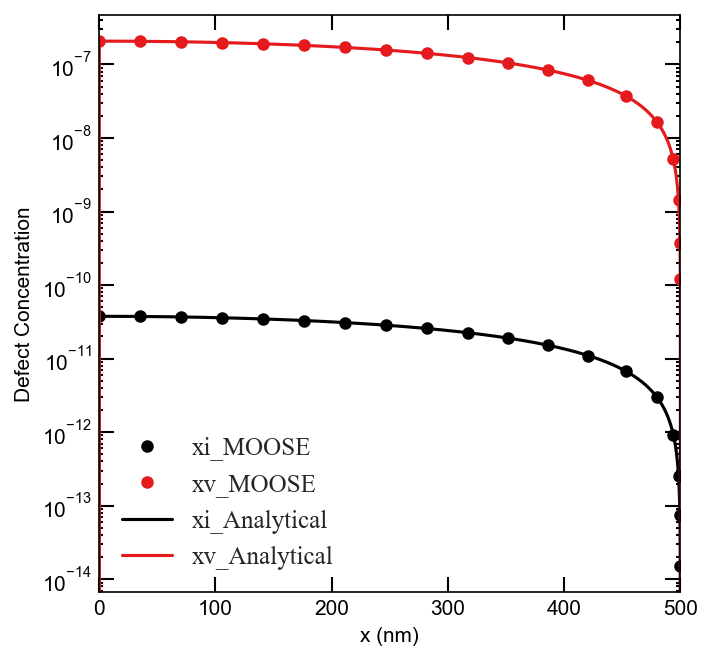
\includegraphics[scale=0.55]{concentration_profiles_MOOSE_Analytical_Neutron_0}
    \caption{Comparison of MOOSE results with analytical solution for spherical grain.}
    \label{figure:concentrations_MOOSE_analytical}
  \end{figure}
  \newpage
  \subsubsection{Concentrations} \hspace{10pt}
  Even though atomic collisions create vacancy-interstitial pairs, following events creates gap between the amount of point defects in favor of vacancies. At steady state condition, there are more vacancies than interstitials in microstructure. Since producing equal amount of point defects is not physically correct, production bias is used to ensure this imbalance in modeling point defects. For unbiased case, as a result of uniform defect production and equilibrium condition at boundaries, the concentration profiles are symmetrical around domain center. The steady state concentration at center is not changing significantly with increasing size as shown in Fig. \ref{figure:concentrations_neutron_0_1e-6}. In case of high neutron dose rate, concentration levels increase, profiles become more stable (see Fig. \ref{figure:concentrations_neutron_0_1e-3}).\\

    \begin{figure}[h!]  %Neutron - 1e-6 dpa/s - %0 Bias rate
      \centering
      \subfloat{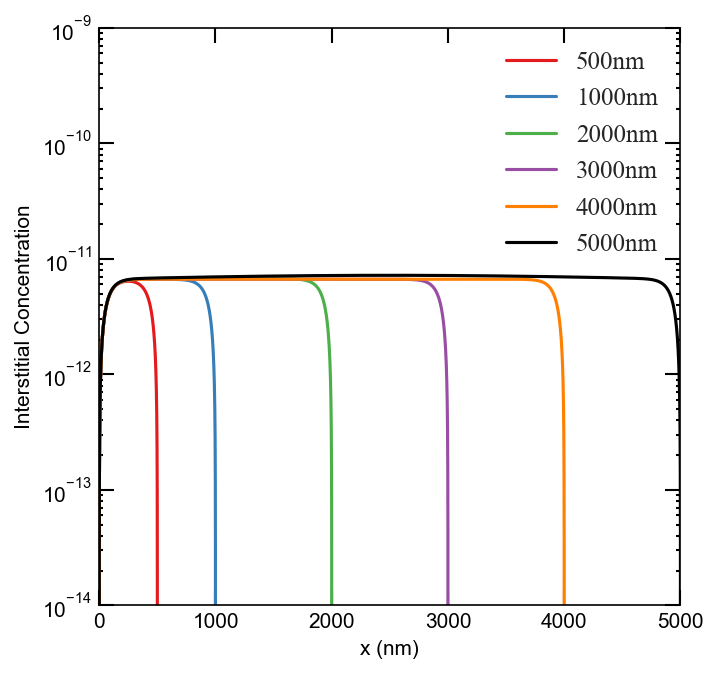
\includegraphics[scale=0.55]{interstitial_concentration_500-5000nm-neutron-0}}
      \qquad
      \subfloat{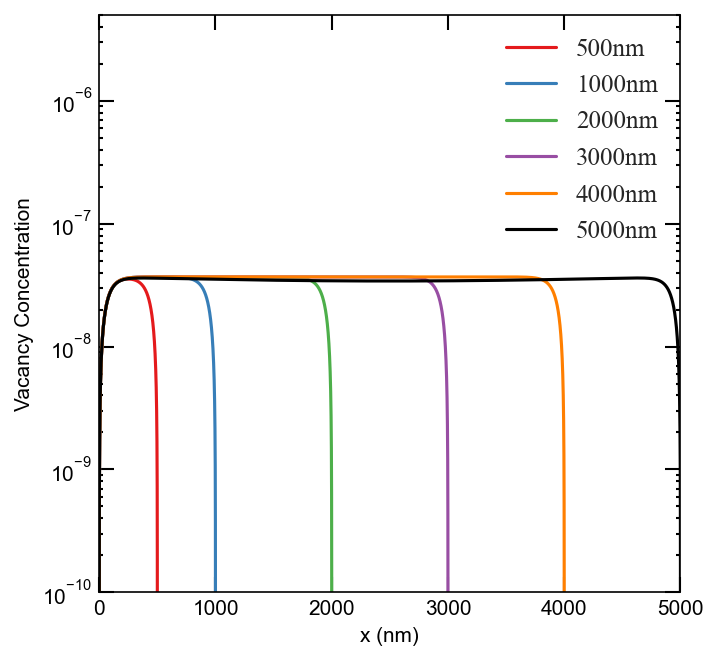
\includegraphics[scale=0.55]{vacancy_concentration_500-5000nm-neutron-0}}
      \caption{Concentration profiles for low dose rate neutron irradation with 0\% Production Bias}
      \label{figure:concentrations_neutron_0_1e-6}
    \end{figure}
    \begin{figure}[h!]  %Neutron - 1e-3 dpa/s - %0 Bias rate
      \centering
      \subfloat{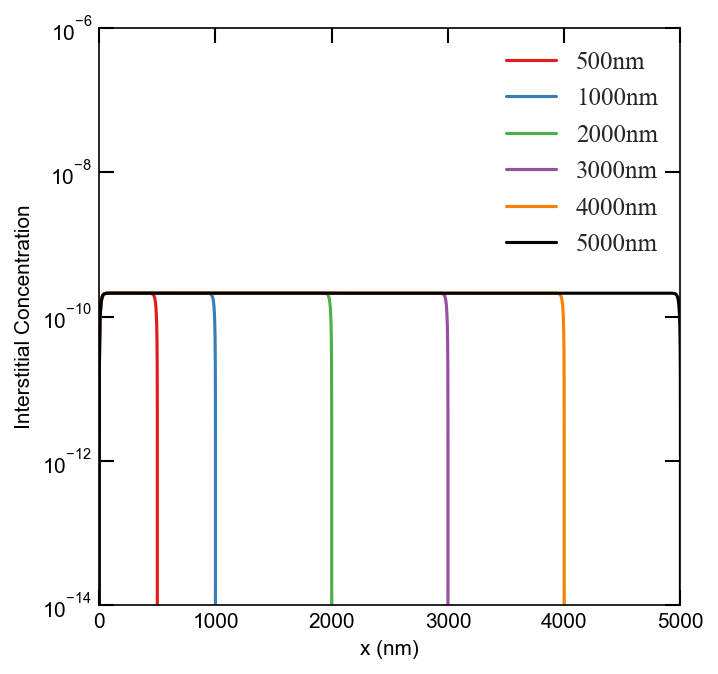
\includegraphics[scale=0.55]{interstitial_concentration_500-5000nm-high_neutron-0}}
      \qquad
      \subfloat{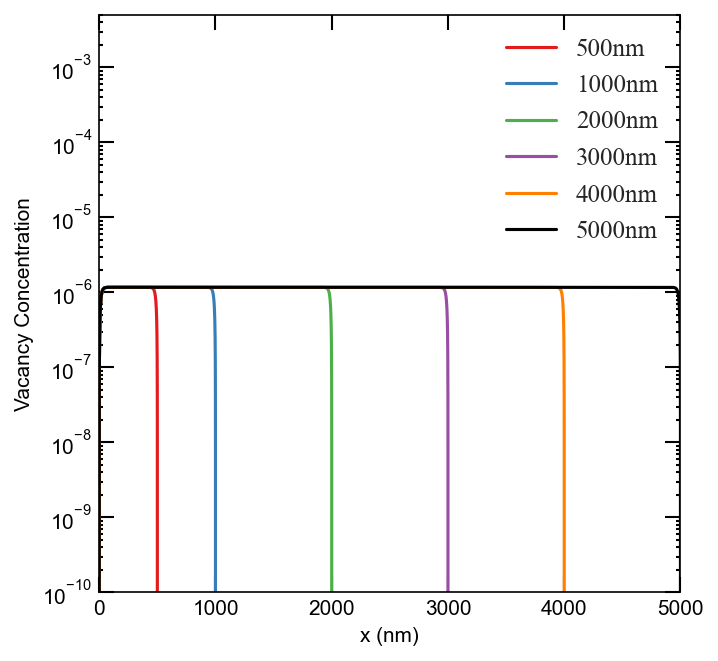
\includegraphics[scale=0.55]{vacancy_concentration_500-5000nm-high_neutron-0}}
      \caption{Concentration profiles for high dose neutron irradation with 0\% Production Bias}
      \label{figure:concentrations_neutron_0_1e-3}
    \end{figure}
    \newpage
     If production bias is applied, the steady state concentration profiles change significantly. The interstitial concentration at center decreases, and its spatial profile turns down after \textit{critical grain size} (${\sim}$1000 nm in Fig. \ref{figure:concentrations_neutron_5_1e-6}). Moreover, the depth of profile gets larger with increasing domain size, which could be explained as acumulation of more interstitial atoms trying to reach equilibrium at boundary. The vacancy concentration, on the other hand, increases proportional to domain size, and its profile having peak at higher concentrations as shown in Fig. \ref{figure:concentrations_neutron_5_1e-6}.\\
    \begin{figure}[h!]  %Neutron - 1e-6 dpa/s - %5 Bias rate
      \centering
      \subfloat{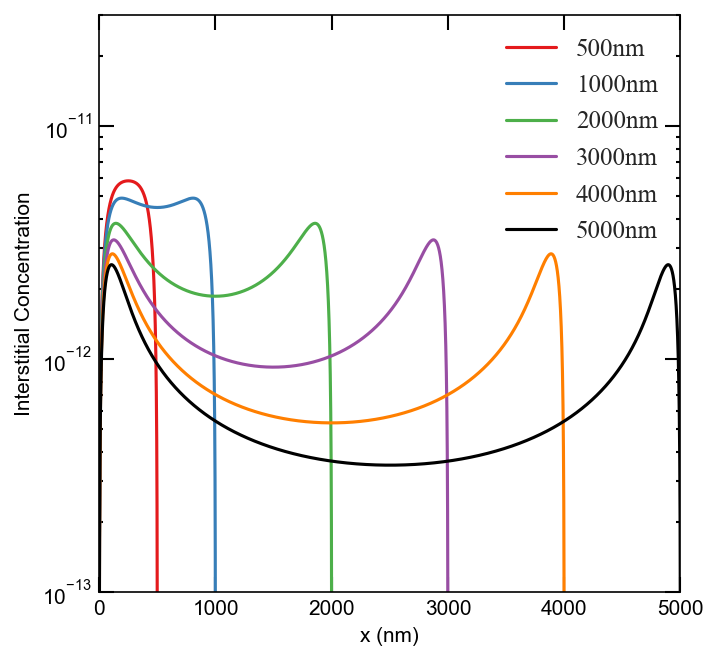
\includegraphics[scale=0.55]{interstitial_concentration_500-5000nm-neutron-5}}
      \qquad
      \subfloat{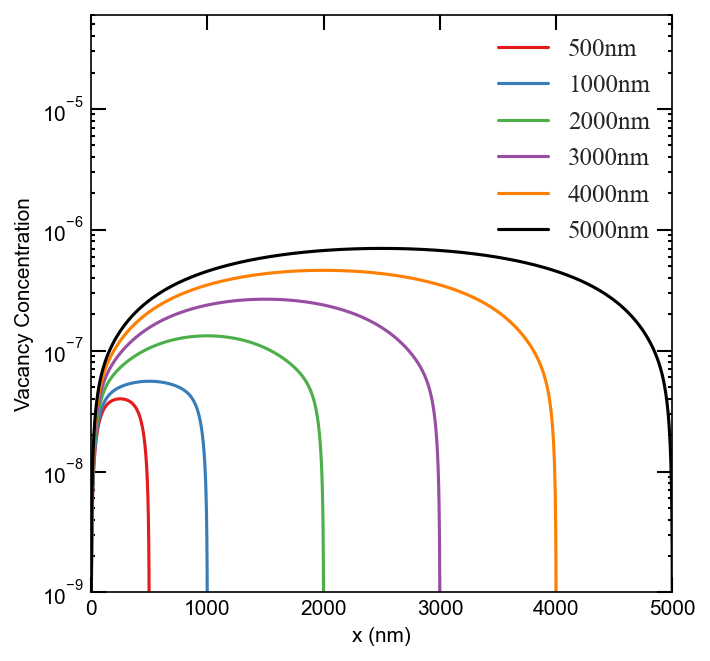
\includegraphics[scale=0.55]{vacancy_concentration_500-5000nm-neutron-5}}
      \caption{Concentration profiles for low dose rate neutron irradation with 5\% Production Bias}
      \label{figure:concentrations_neutron_5_1e-6}
    \end{figure}\\

    Similar to unbiased case, average concentration levels increases with dose rate. But, the most important effect of high neutron dose rate is causing the interstitial concentration profile to flip in smaller domain sizes than 500 nm (see Fig. \ref{figure:concentrations_neutron_5_1e-3}).\\
    \begin{figure}[htb!]  %Neutron - 1e-3 dpa/s - %5 Bias rate
      \centering
      \subfloat{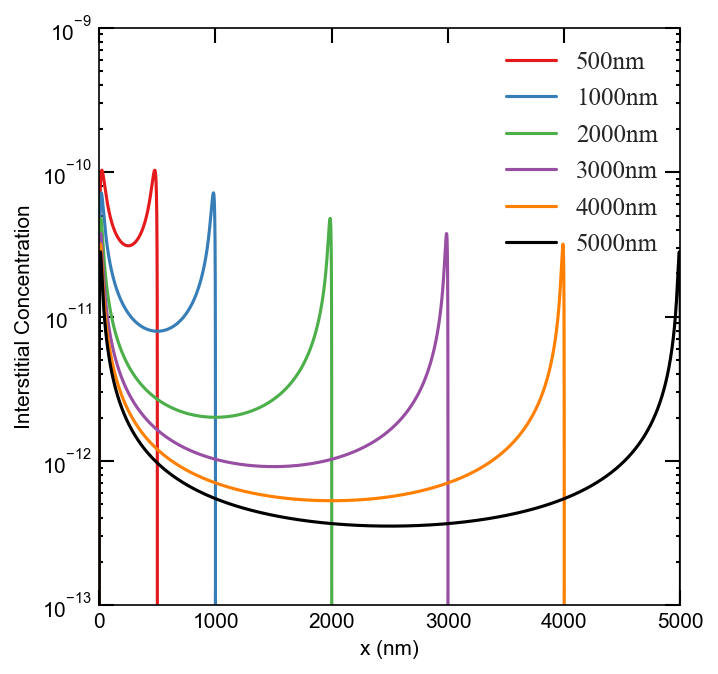
\includegraphics[scale=0.55]{interstitial_concentration_500-5000nm-high_neutron-5}}
      \qquad
      \subfloat{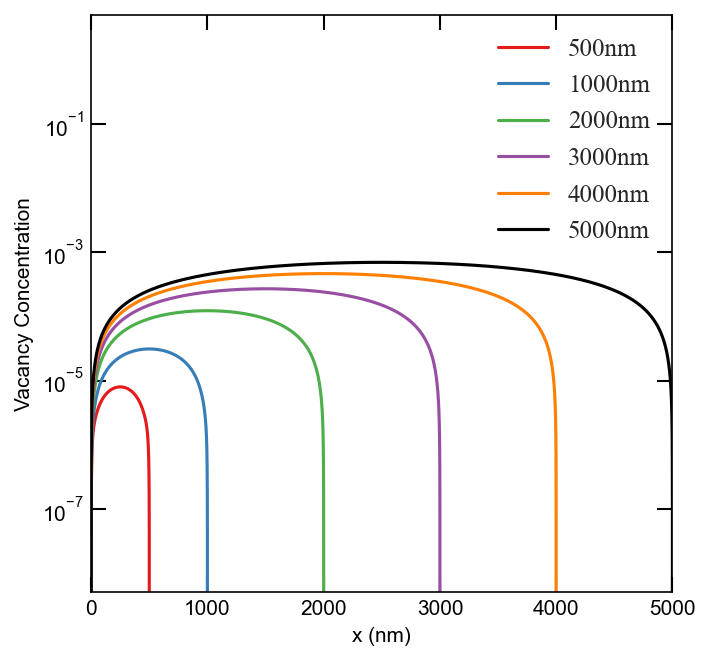
\includegraphics[scale=0.55]{vacancy_concentration_500-5000nm-high_neutron-5}}
      \caption{Concentration profiles for high dose neutron irradation with 5\% Production Bias}
      \label{figure:concentrations_neutron_5_1e-3}
    \end{figure}

    \newpage
    \subsubsection{Supersaturation} \hspace{10pt}
    Supersaturation is a condition that the actual concentration of point defect is larger than its equilibrium concentration. The opposite condition is called undersaturation which is being smaller than equilibrium concentration. In both cases, the system is not at the minimum free energy. Both vacancies and interstitials could be supersaturated, then aggiomerate into voids or discs of interstitial atoms. These can produce stacking faults in crystal microstructure.

    The effective vacancy supersaturation, ${S_v}$ is calculated by using following equation,\cite{was2016}\\

    \begin{equation}
      \begin{aligned}
        &S_v=\frac{D_vC_v-D_iC_i}{D_vC_v^e}\\
      \end{aligned}
    \end{equation}\\

    The vacancy supersaturation curves for biased neutron irradation is given in Fig. \ref{figure:vacancy_supersaturation_neutron_5}. Since the defect concentrations are symmetrical for neutron irradation, supersaturation curves are also symmetrical around domain center. The plot shows a non-linear increase in supersaturation values as domain gets larger.
      \begin{figure}[h!]  %Nuetron - Vacancy Supersaturation - 5% Bias
        \centering
        \subfloat{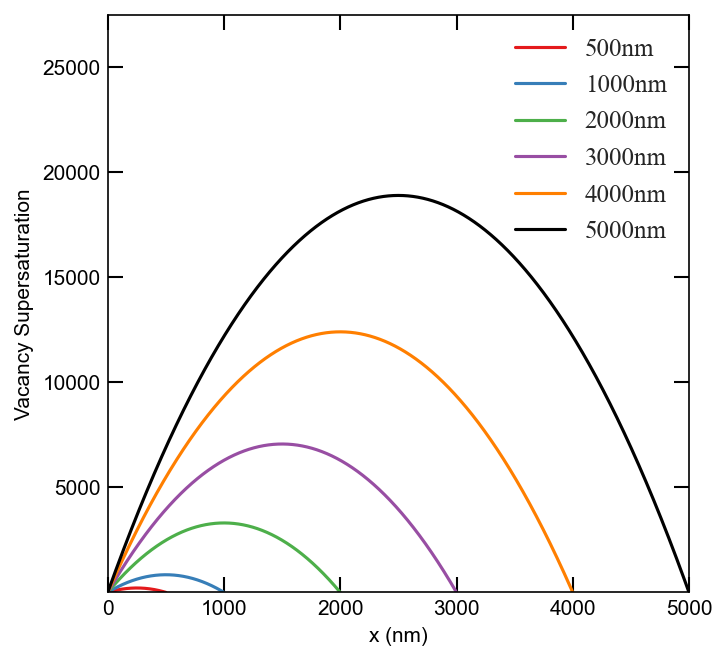
\includegraphics[scale=0.55]{super_saturation_500-5000nm-neutron-5}}
        \qquad
        \subfloat{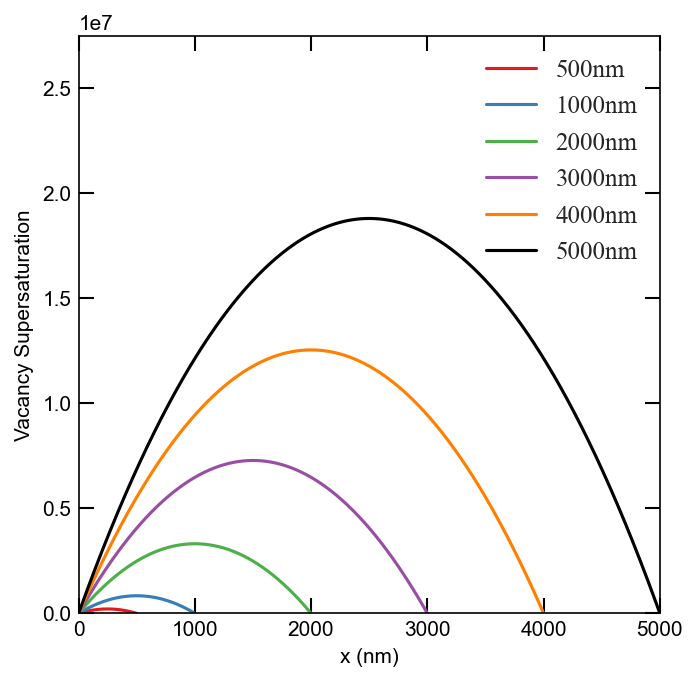
\includegraphics[scale=0.55]{super_saturation_500-5000nm-high_neutron-5}}
        \caption{Vacancy Supersaturation profiles for low and high dose neutron irradation with 5\% Production Bias}
        \label{figure:vacancy_supersaturation_neutron_5}
      \end{figure}

    \subsubsection{Sink Strengths} \hspace{10pt}
    The sink reaction term in Eq. \ref{equation:point_defect_equations_sink_strength} represents the total loss of point defects to sinks that are voids and dislocations within the domain. It can be written in expanded form as below,

    \begin{equation}
      \begin{aligned}
        &k^2DC=(Z\rho_d+4\pi r_h\rho_h)DC\\
      \end{aligned}
    \end{equation}\\
    Similarly, grain boundary sink strength can be calculated by considering total flow of point defect to grain boundary.

    \begin{equation}
      \begin{aligned}
        &F=Z_{gb}DC_0\\
        &Z_{gb}=\frac{F}{DC_0}\\
      \end{aligned}
      \end{equation}\\

    where ${F}$ is total flow at grain boundary, ${Z_{gb}}$ is grain boundary sink strength, ${D}$ is diffusion coefficient and ${C_0}$ is defect concentration at the domain center.\\\\
    The total flow at boundary is equal to multiplication of surface area and current as below,\\

    \begin{equation}
      \begin{aligned}
        &F=-\bigg(4\pi r^2D\frac{\partial C(r)}{\partial r}\bigg)_{r=a}\\
      \end{aligned}
    \end{equation}\\
    The total grain boundary sink strength, ${k^2_{gb}}$ is calculated by multiplying ${Z_{gb}}$ by the grain density, ${\rho_{gb}}$.\cite{heald1977}
    \begin{equation}
      \begin{aligned}
        &\rho_{gb}=\frac{6}{\pi d^3}\\
        &k^2_{gb}=\rho_{gb}Z_{gb}\\
      \end{aligned}
    \end{equation}

    where ${d}$ is diameter of the grain, ${d=2a}$\\\\
    Grain boundary sink strengths, ${Z_{gb}}$ and ${k_{gb}}$, is calculated analytically by substituting Eq.  \ref{equation:spherical_grain_analytical_solution} into expressions above. Thus, grain boundary sink strengths are associated with the domain sink strength, ${k^2}$.\cite{heald1977}

    \begin{equation}
      \begin{aligned}
        &C_0=C(r=0)=\frac{K_0}{Dk^2}\bigg(1-\frac{ka}{\sinh{ka}}\bigg)\\\\
        &F=-\bigg(4\pi r^2D\frac{\partial C(r)}{\partial r}\bigg)_{r=a}=\frac{4\pi aK_0}{k^2}\bigg(ka\coth{ka}-1\bigg)\\
      \end{aligned}
    \end{equation}\\
    So that, grain boundary sink strengths are
    \begin{equation}
      \begin{aligned}
        &Z_{gb}=4\pi a\bigg(\frac{ka\cosh ka-\sinh ka}{\sinh ka-ka}\bigg)\\
        &k^2_{gb}=\frac{12}{d^2}\bigg(\frac{ka\cosh ka-\sinh ka}{\sinh ka-ka}\bigg)\\
      \end{aligned}
    \end{equation}\\

    Using appropriate diffusion coefficient (${D}$), domain sink strength (${k^2}$) and concentration (${C_0}$) will give  relevant sink strengths. The analytical expressions for each defect type given by following equations

    \begin{equation}
      \begin{aligned}
        &Z_{gb,i}=4\pi a\bigg(\frac{k_ia\cosh k_ia-\sinh k_ia}{\sinh k_ia-k_ia}\bigg)\\
        &k^2_{gb,i}=\frac{12}{d^2}\bigg(\frac{k_ia\cosh k_ia-\sinh k_ia}{\sinh k_ia-k_ia}\bigg)\\\\
        &Z_{gb,v}=4\pi a\bigg(\frac{k_va\cosh k_va-\sinh k_va}{\sinh k_va-k_va}\bigg)\\
        &k^2_{gb,v}=\frac{12}{d^2}\bigg(\frac{k_va\cosh k_va-\sinh k_va}{\sinh k_va-k_va}\bigg)\\
      \end{aligned}
    \end{equation}\\

  The results of bencmark problem, previously discussed in Fig. \ref{figure:concentrations_MOOSE_analytical}, can also be used to validate MOOSE sink strength calculations. Table \ref{table:sink_strengths_calculations} show the comparison of calculations.
    \begin{table}[h!]
      \centering
      \caption{Comparison of sink strength calculations}
      \label{table:sink_strengths_calculations}
      \begin{tabular}{ ||p{2cm}|p{3cm}|p{3cm}||  }
         \hline
          & MOOSE & Analytical\\
         \hline\hline\hline
         ${Z_{gb,i}}$  & 1.257206e-05 m & 1.257332e-05 m\\
         ${Z_{gb,v}}$  & 1.256941e-05 m & 1.257332e-05 m\\
         ${k_{gb,i}}$  & 2.401086e+13 m^{-2} & 2.401327e+13 m^{-2}\\
         ${k_{gb,v}}$  & 2.400580e+13 m^{-2} & 2.401327e+13 m^{-2}\\
         \hline
      \end{tabular}
    \end{table}
    \newpage
    Sink strength plots are presented in Fig. \ref{figure:sink_strengths_neutron_5_1e-6} and \ref{figure:sink_strengths_neutron_5_1e-3}. The effect of flipping behavior is not visible in grain boundary sink strength, ${Z^{gb}}$ plot, but in total grain boundary sink strength, ${k^2}$ plot, there is a significant change on ${k^2_i}$ after critical grain size of ${\sim}$1000 nm. In high dose rate plot, the critical grain size is seen clearly around at ${\sim}$250 nm.
      % \begin{figure}[h!]  %Sink Strength - Neutron 1e-6 dpa/s - 0% Bias rate
      %   \centering
      %   \subfloat{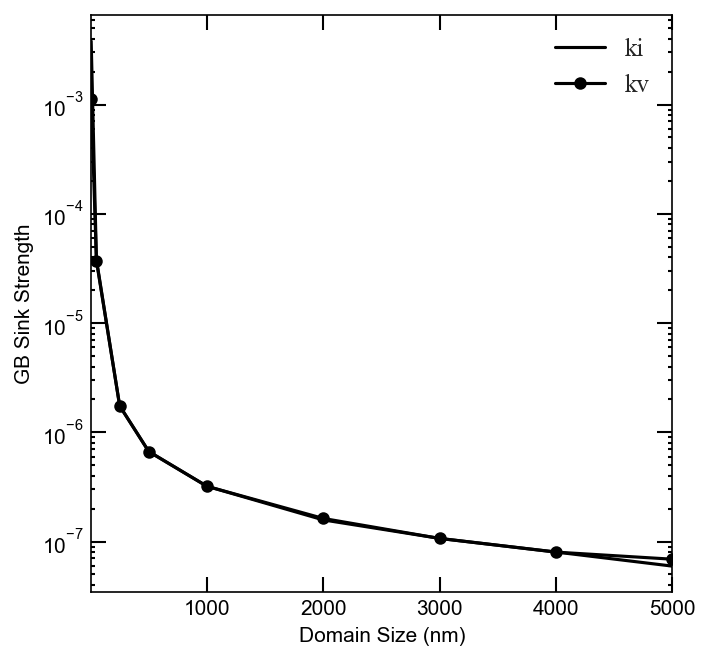
\includegraphics[scale=0.55]{sink_strength_moose_neutron_0_k}}
      %   \qquad
      %   \subfloat{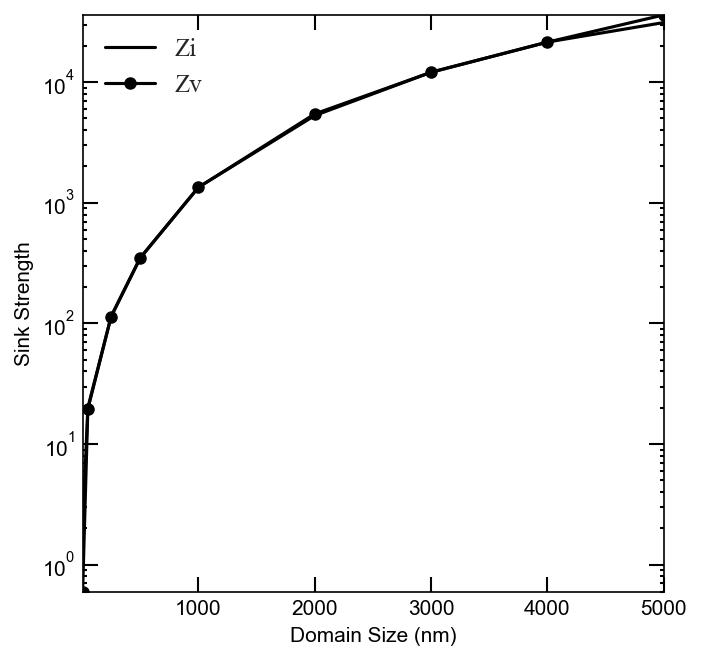
\includegraphics[scale=0.55]{sink_strength_moose_neutron_0_Z}}
      %   \caption{Sink Strengths for low dose rate neutron irradiation with 0\% Production Bias}
      %   \label{figure:sink_strengths_neutron_0_1e-6}
      % \end{figure}
      \begin{figure}[h!]  %Sink Strength - Neutron 1e-6 dpa/s - 5% Bias rate
        \centering
        \subfloat{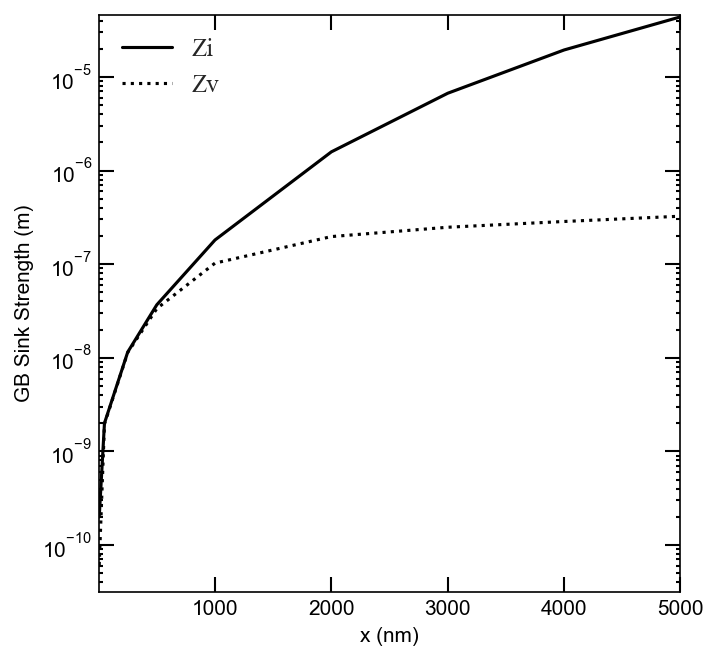
\includegraphics[scale=0.55]{sink_strength_moose_neutron_5_Z_scaled}}
        \qquad
        \subfloat{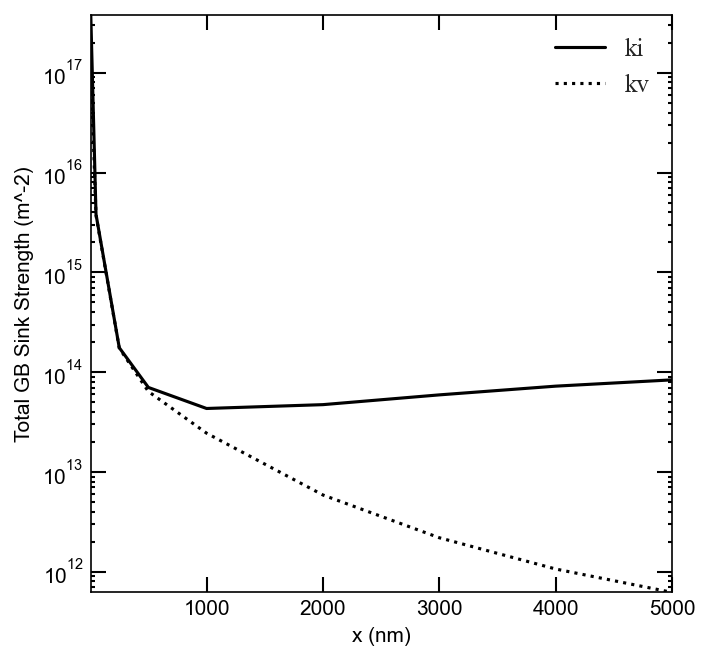
\includegraphics[scale=0.55]{sink_strength_moose_neutron_5_k_scaled}}
        \caption{Sink Strengths for low dose rate neutron irradation with 5\% Production Bias}
        \label{figure:sink_strengths_neutron_5_1e-6}
      \end{figure}
      \begin{figure}[h!]  %Sink Strength - Neutron 1e-6 dpa/s - 5% Bias rate
        \centering
        \subfloat{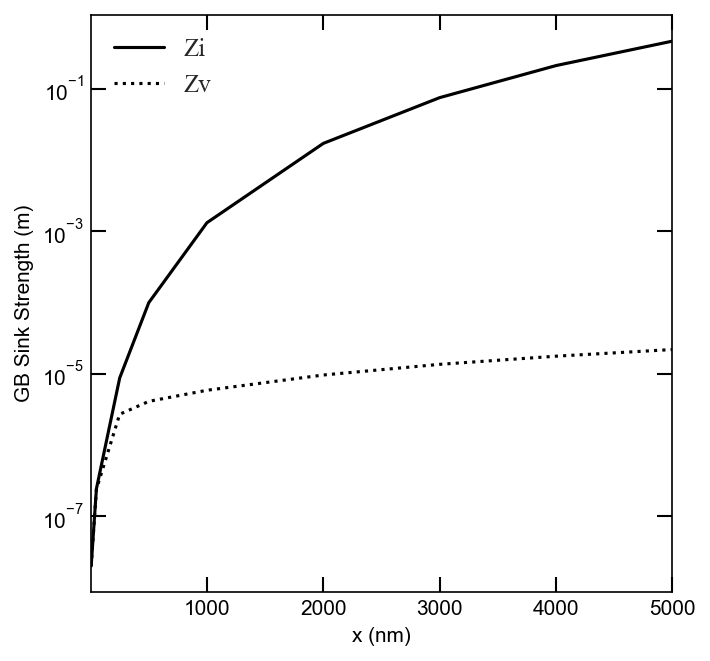
\includegraphics[scale=0.55]{sink_strength_moose_high_neutron_5_Z_scaled}}
        \qquad
        \subfloat{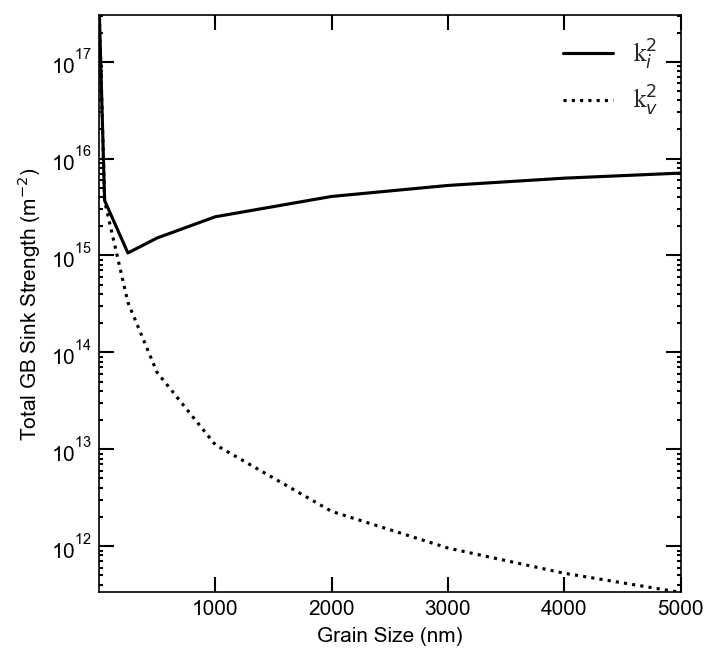
\includegraphics[scale=0.55]{sink_strength_moose_high_neutron_5_k_scaled}}
        \caption{Sink Strengths for high dose rate neutron irradation with 5\% Production Bias}
        \label{figure:sink_strengths_neutron_5_1e-3}
      \end{figure}
  \newpage
  \subsection{Ion Irradiation} \hspace{10pt}
  Unlike neutrons, ions have relatively narrow energy channel width which is almost monoenergetic. Furthermore, they cannot penetrate through material too much because of their high energy loss in collisions. These characteristic causes a non-uniform defect production profile. The defect production profile used for ion irradation simulations are shown in Fig. \ref{figure:defect_production}. The dose rate, K\textsubscript{0} and domain size (1000 nm) would be scaled for different cases, but the profile is going to stay unchanged.
    \begin{figure}[h!]  %Ion irradation
      \centering
      \subfloat{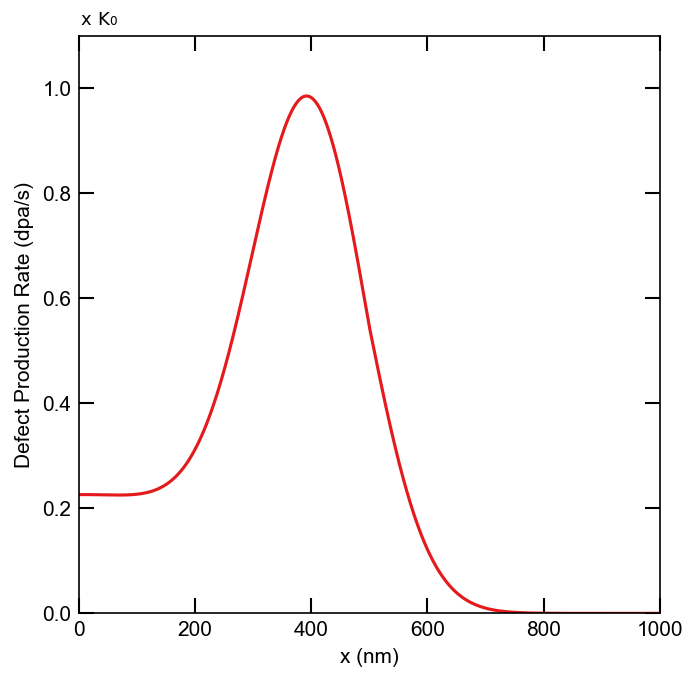
\includegraphics[scale=0.27]{defect_production}}
      \qquad
      \caption{Defect production profile for ion irradation.}
      \label{figure:defect_production}
    \end{figure}
    \subsubsection{Concentrations} \hspace{10pt}
    The effect of defect production distribution is the first thing that can be observed easily on concentration profiles. Since, all defect production profiles having peak at around half of the domain, the concentration profiles are also showing the same behavior and reaching maximum at the center of domain, then waning through boundaries.

    If production bias is zero, maximum concentration that point defects can reach is equal for all different domain sizes shown in Fig. \ref{figure:concentrations_ion_0_1e-6}. High ion dose rate is scaling up the concentration levels without making a significant change in profiles (see Fig. \ref{figure:concentrations_ion_0_1e-3}).
      \begin{figure}[h!]  %Ion - 1e-3 dpa/s - %0 Bias rate
        \centering
        \subfloat{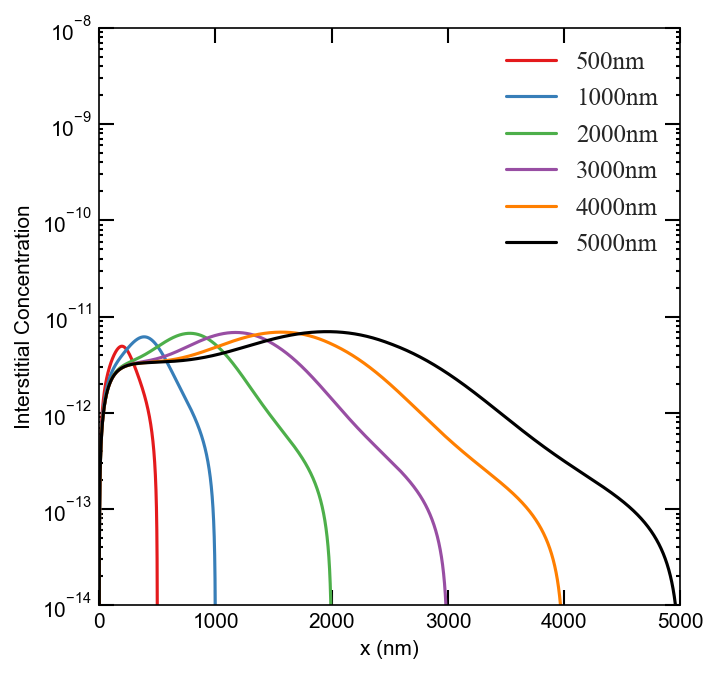
\includegraphics[scale=0.55]{interstitial_concentration_500-5000nm-low_ion-0}}
        \qquad
        \subfloat{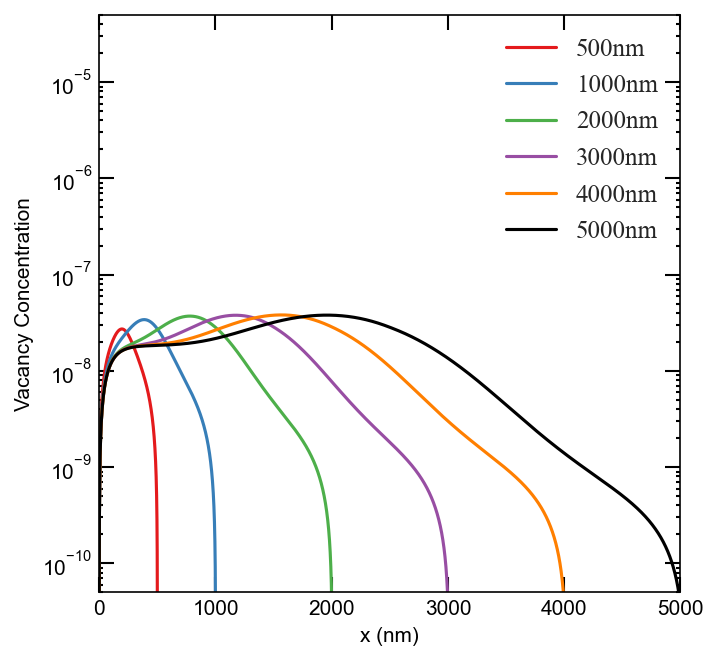
\includegraphics[scale=0.55]{vacancy_concentration_500-5000nm-low_ion-0}}
        \caption{Concentration profiles for low dose ion irradation with 0\% Production Bias}
        \label{figure:concentrations_ion_0_1e-6}
      \end{figure}
      \begin{figure}[h!]  %Ion - 1e-6 dpa/s - %0 Bias rate
        \centering
        \subfloat{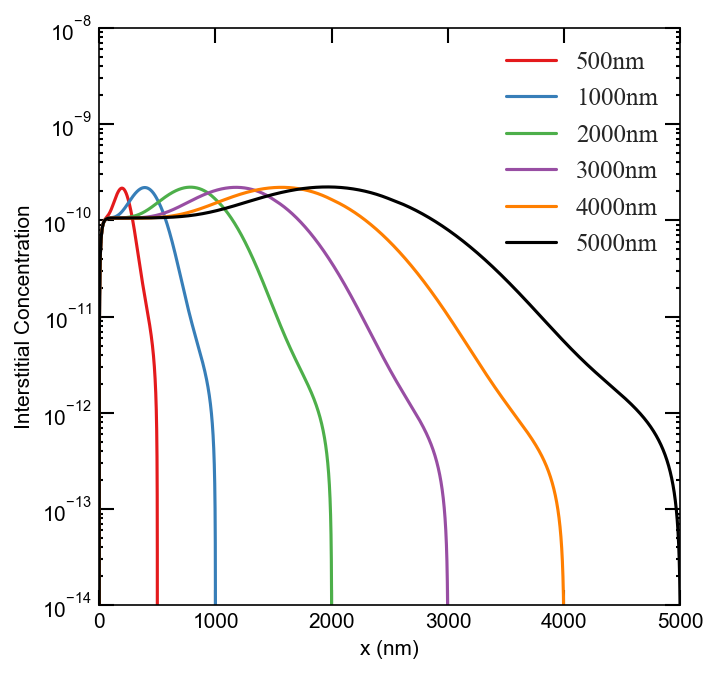
\includegraphics[scale=0.55]{interstitial_concentration_500-5000nm-ion-0}}
        \qquad
        \subfloat{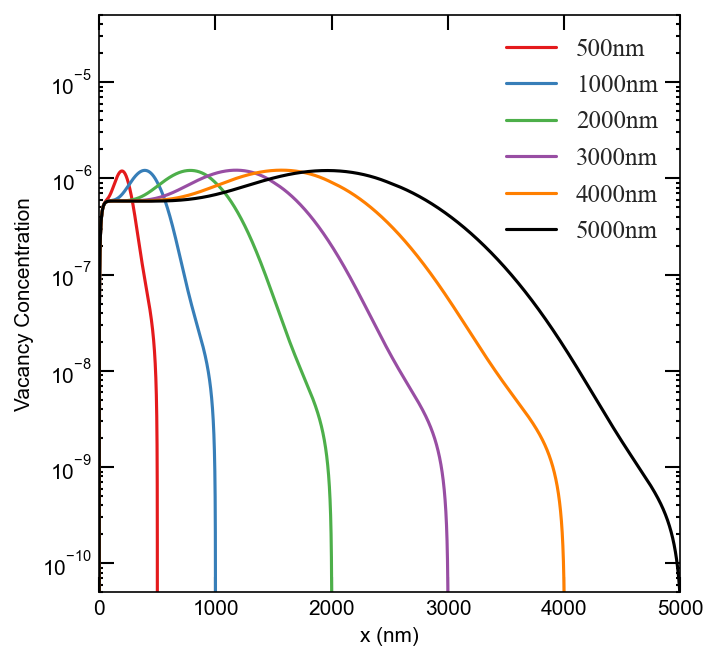
\includegraphics[scale=0.55]{vacancy_concentration_500-5000nm-ion-0}}
        \caption{Concentration profiles for high dose rate ion irradiation with 0\% Production Bias}
        \label{figure:concentrations_ion_0_1e-3}
      \end{figure}
      \newpage
      In case of applying production bias, profiles become completely different. Although the flipping behavior observed in neutron irradation case is also visible in ion irradation case, the non-uniform defect production causes asymmetrical interstitial concentration profile in Fig. \ref{figure:concentrations_ion_5_1e-6}. The vacancy concentration profiles also become asymmetrical and shift up with increasing domain size. Increasing ion dose rate from 1e-6 dpa/s to 1e-3 dpa/s reduces the effect of defect production profile as well as critical grain size to flip (see Fig. \ref{figure:concentrations_ion_5_1e-3}).
      \begin{figure}[h!]  %Ion - 1e-3 dpa/s - %5 Bias rate
        \centering
        \subfloat{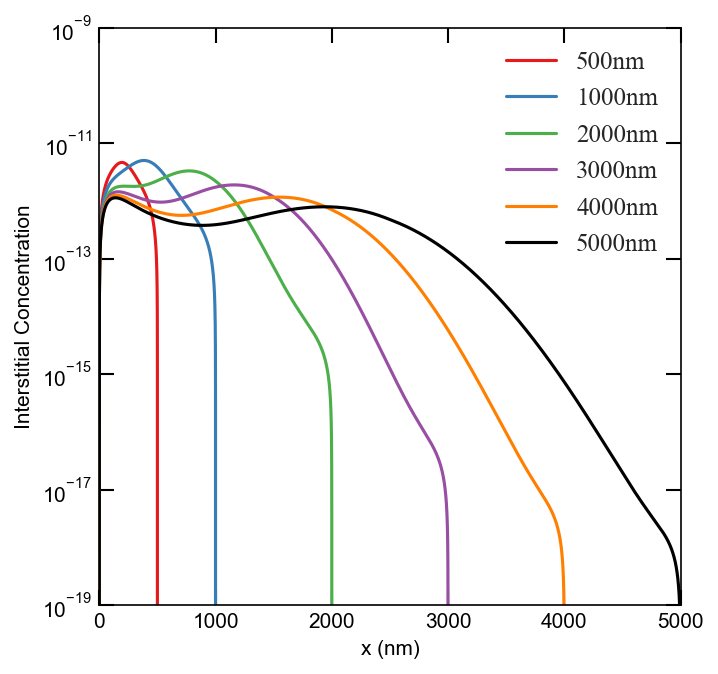
\includegraphics[scale=0.55]{interstitial_concentration_500-5000nm-low_ion-5}}
        \qquad
        \subfloat{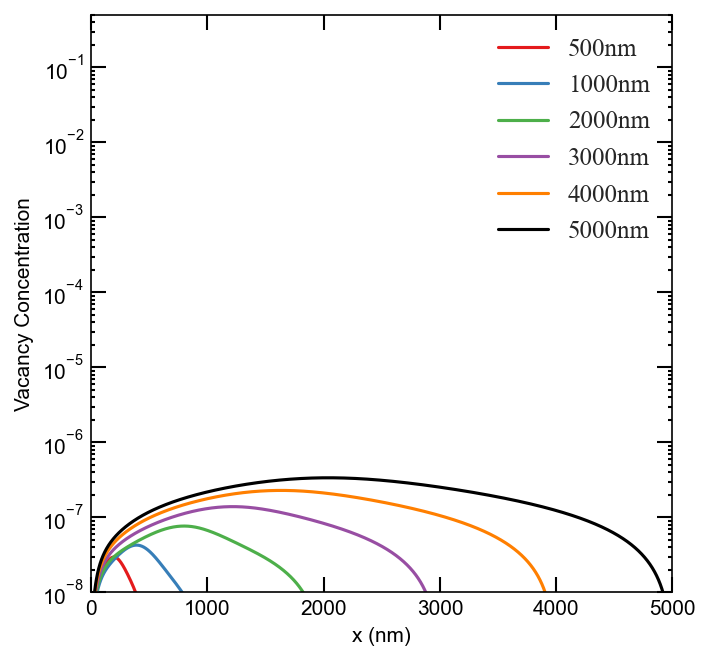
\includegraphics[scale=0.55]{vacancy_concentration_500-5000nm-low_ion-5}}
        \caption{Concentration profiles for low dose ion irradation with 5\% Production Bias}
        \label{figure:concentrations_ion_5_1e-6}
      \end{figure}
      \begin{figure}[h!]  %Ion - 1e-6 dpa/s - %5 Bias rate
        \centering
        \subfloat{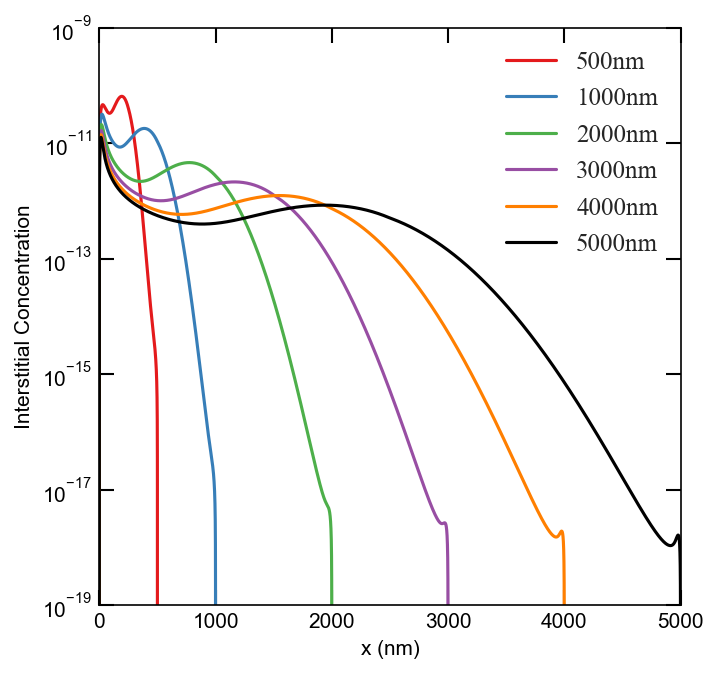
\includegraphics[scale=0.55]{interstitial_concentration_500-5000nm-ion-5}}
        \qquad
        \subfloat{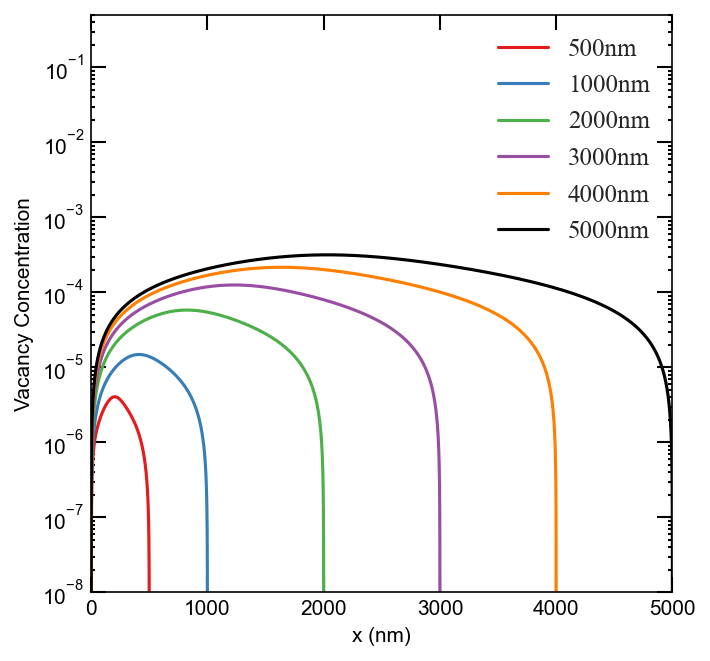
\includegraphics[scale=0.55]{vacancy_concentration_500-5000nm-ion-5}}
        \caption{Concentration profiles for high dose rate ion irradation with 5\% Production Bias}
        \label{figure:concentrations_ion_5_1e-3}
      \end{figure}

    \newpage
    \subsubsection{Supersaturation} \hspace{10pt}

    The vacancy supersaturation curves for ion irradation case are quite similar to ones for neutron irradation case. The only difference is the asymmetrical shape of curves originates from concentration profiles. The non-linear increase in supersaturation values as domain gets larger is observed for ion irradation too.
      \begin{figure}[h!]  %Ion - %5 Bias rate
        \centering
        \subfloat{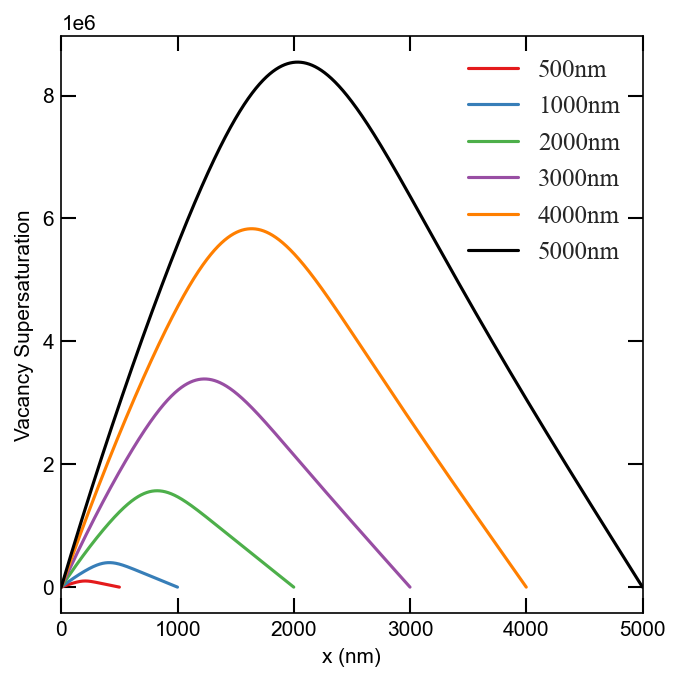
\includegraphics[scale=0.55]{super_saturation_500-5000nm-ion-5}}
        \qquad
        \subfloat{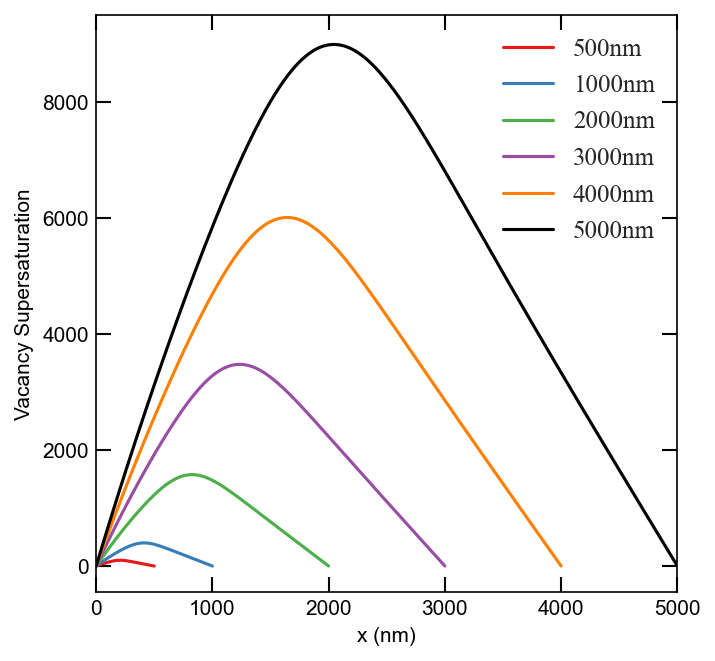
\includegraphics[scale=0.55]{super_saturation_500-5000nm-low_ion-5}}
        \caption{Vacancy Supersaturation profiles for low dose and ion irradation with 5\% Production Bias}
        \label{figure:vacancy_supersaturation_ion_5}
      \end{figure}
    \subsubsection{Sink Strengths} \hspace{10pt}
    The sink strengths are directly related to concentration at center and flow at boundary. The change in centerline defect concentrations are not as considerable as neutron case. So, the flow or flux at boundary becomes more dominant on sink strength profiles (see Fig. \ref{figure:sink_strengths_ion_5_1e-6} and \ref{figure:sink_strengths_ion_5_1e-3}).
      % \begin{figure}[h!]  %Sink Strength - ion 1e-3 dpa/s - 0% Bias rate
      %   \centering
      %   \subfloat{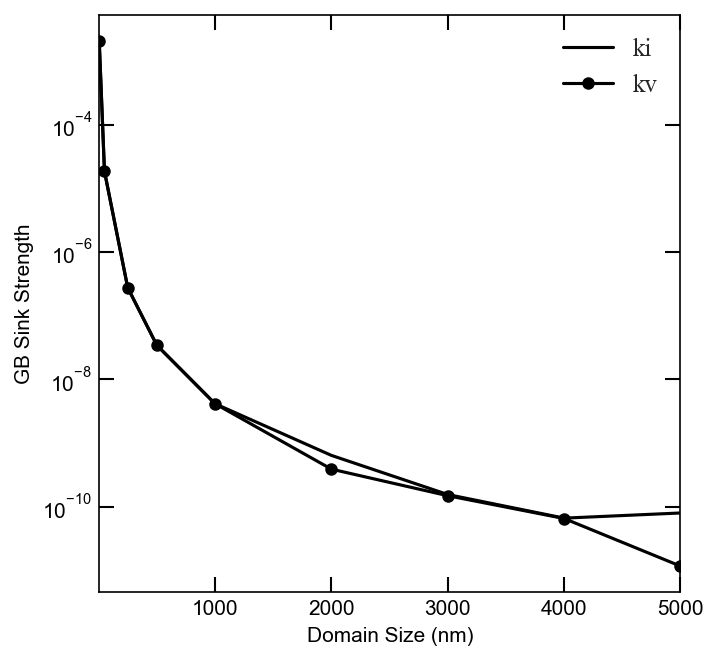
\includegraphics[scale=0.55]{sink_strength_moose_ion_0_k}}
      %   \qquad
      %   \subfloat{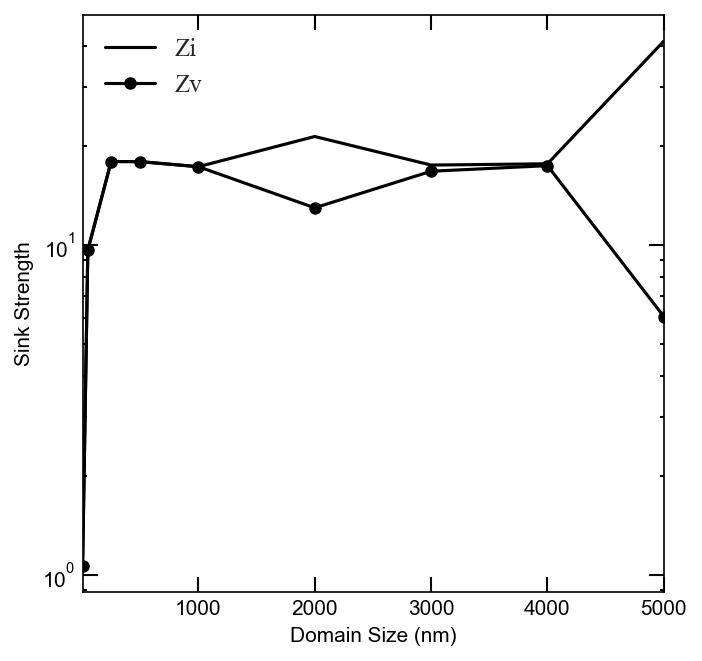
\includegraphics[scale=0.55]{sink_strength_moose_ion_0_Z}}
      %   \caption{Sink Strengths for low dose ion irradation with 0\% Production Bias}
      %   \label{figure:sink_strengths_ion_0_1e-6}
      % \end{figure}
      \begin{figure}[h!]  %Sink Strength - ion 1e-6 dpa/s - 5% Bias rate
        \centering
        \subfloat{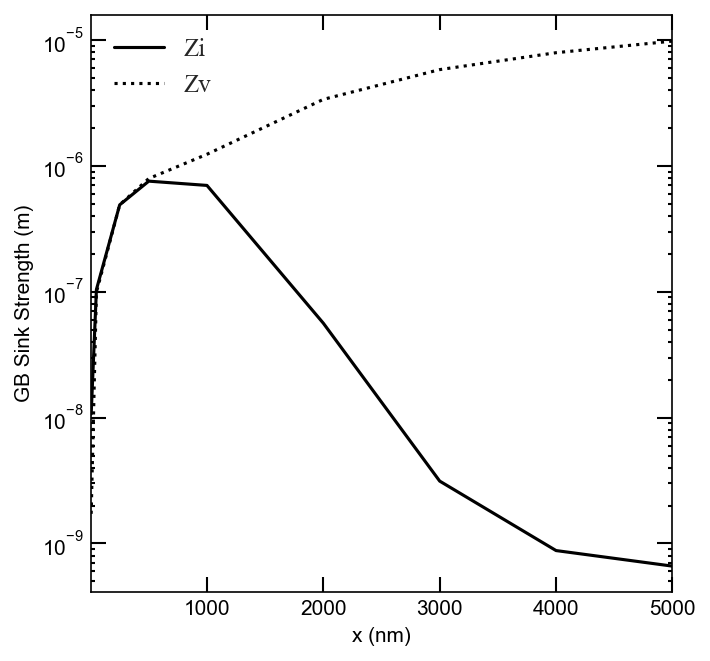
\includegraphics[scale=0.55]{sink_strength_moose_low_ion_5_Z_scaled}}
        \qquad
        \subfloat{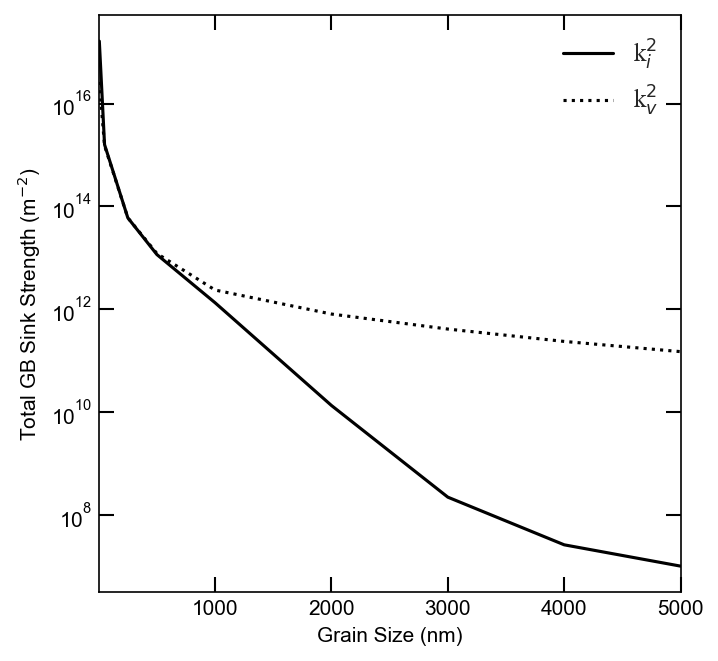
\includegraphics[scale=0.55]{sink_strength_moose_low_ion_5_k_scaled}}
        \caption{Sink Strengths for low dose rate ion irradiation with 5\% Production Bias}
        \label{figure:sink_strengths_ion_5_1e-6}
      \end{figure}
      \begin{figure}[h!]  %Sink Strength - ion 1e-3 dpa/s - 5% Bias rate
        \centering
        \subfloat{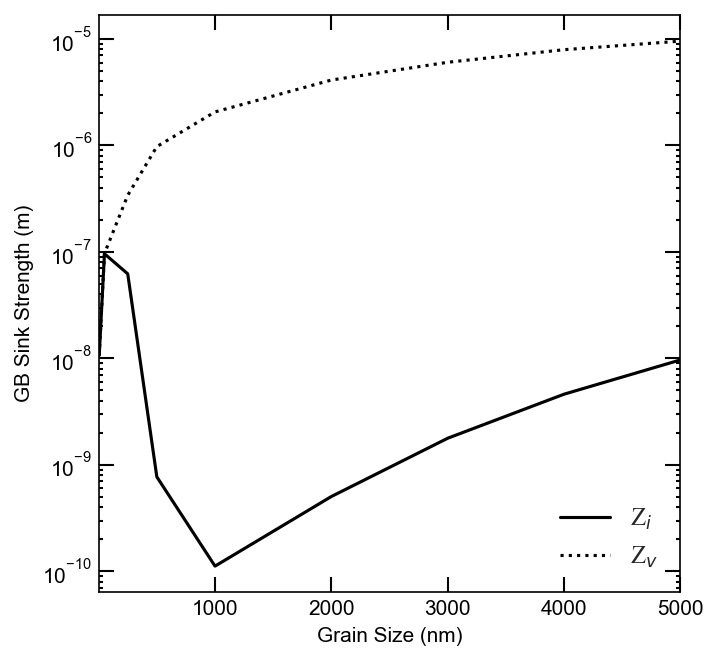
\includegraphics[scale=0.55]{sink_strength_moose_ion_5_Z_scaled}}
        \qquad
        \subfloat{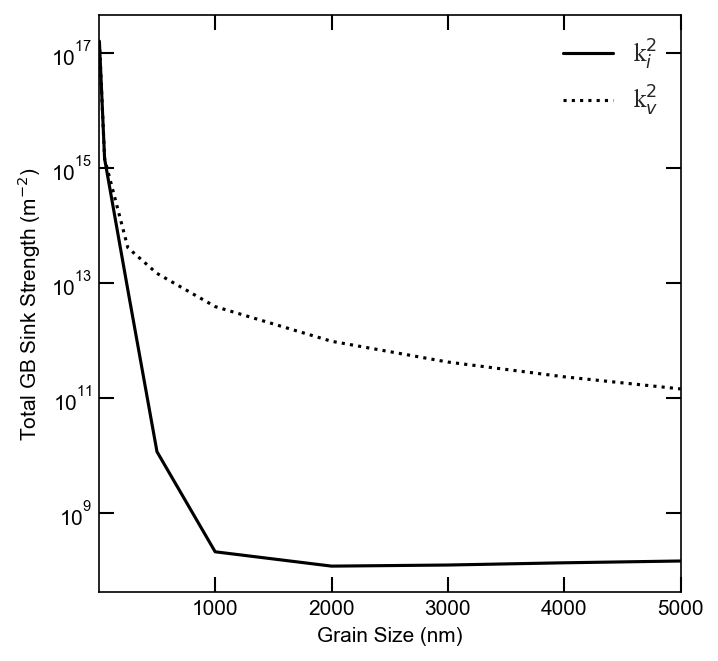
\includegraphics[scale=0.55]{sink_strength_moose_ion_5_k_scaled}}
        \caption{Sink Strengths for high dose rate ion irradiation with 5\% Production Bias}
        \label{figure:sink_strengths_ion_5_1e-3}
      \end{figure}


% In nano-scale case, since the domain size is not big enough, the boundaries become
% closer to each other. This causes point defects to reach sinks before they react with each other
% and recombination plateau to disappear as it can be seen in Fig. 2. The nanoscale case acts like
% a high-sink and high-temp condition case despite its low-sink and low-temperature. Therefore,
% change in production bias does not have a significant effect on average concentration behavior
% in nanoscale
%
% On the other hand, in micro-scale case, the domain has reasonable size, and thus
% boundaries are far from each other. This provides defects more time to accumulate inside the
% domain and recombine with each other after they reach a specific concentration. Figure 3
% clearly shows the effect of production bias on average concentration.
%
% Effect of production bias on spatial profile of defect concentrations for nanoscale is
% shown in Figure 4. The results seem not affected too much because of the same reasons
% mentioned previously for average concentration.
%
% The micro-scale results (Fig. 5) are quite interesting and worth to think over. The
% concentration profiles of interstitials for 0.1%, 5% and 10% cases are flipped over. A closer look
% at evolution of 5% case over time in Fig. 6, after the end of quasi-steady-state region (t=10 -4 s in
% Fig 3.), the average interstitial concentration starts to decrease as they segregate through sinks.
% At steady state, the average interstitial concentration becomes minimum at the center and
% maximum near boundaries because of segregation.
%
% The defect production rate (K 0 ) is the source term in point defect equations and has a
% significant effect on concentrations.
% In nano-scale case, the average concentration behavior is like high-sink density behavior
% because of narrow domain. But, when the defect production rate increases, the average
% concentration is shifted upward, and interstitial and vacancy average concentrations get closer
% to each other because the production compensates more absorption at sinks than previous.
% Based on this, if the production rate increased sufficiently, the recombination zone would
% appear again in nano-scale domain.

\newpage
\section{Conclusion} \hspace{10pt}

The rate theory equations resolve the temporal and spatial concentration profiles of point defects. The behavior of concentration distributions are controlled by parameters given in equation, representing their reactions and diffusion in domain. According to the results obtained in this study, the combination of production bias, production dose rate, production profile and domain size determine whether the steady state point defect concentration profile is symmetrical, flipped or both. There is always a critical value for parameters that could change the defect concentration profile entirely.

% An online tool could be created to play with different parameters.
% \begin{thebibliography}{00}
% \bibitem{b2} Garry S. Was.
% \end{thebibliography}
\addcontentsline{toc}{section}{References}
\bibliographystyle{unsrt}
\bibliography{ref}

\end{document}
